\documentclass[12pt]{standalone}
\usepackage{tikz-feynman}

\begin{document}
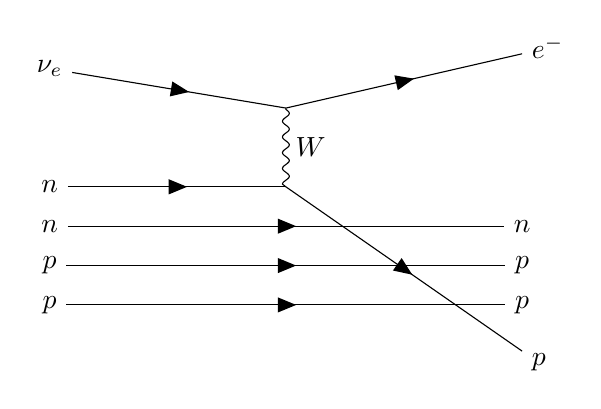
\begin{tikzpicture}
    \begin{feynman}
        \vertex (e1) {$\nu_e$};
        \vertex [below right=5mm and 30mm of e1] (e2);
        \vertex [above right=5mm and 30mm of e2] (e3) {$e^-$};
        \vertex [below=of e1] (hitnuc1) {$n$};
        \vertex [right=30mm of hitnuc1] (hitnuc2);
        \vertex [below right=20mm and 30mm of hitnuc2] (hitnuc3) {$p$};
        \vertex [below=5mm of hitnuc1] (nuc1) {$n$};
        \vertex [right=60mm of nuc1] (nuc1p) {$n$};
        \vertex [below=5mm of nuc1] (nuc2) {$p$};
        \vertex [right=60mm of nuc2] (nuc2p) {$p$};
        \vertex [below=5mm of nuc2] (nuc3) {$p$};
        \vertex [right=60mm of nuc3] (nuc3p) {$p$};

        \diagram* {
            (e1) -- [fermion] (e2) -- [fermion] (e3),
            (e2) -- [boson, edge label=\(W\)] (hitnuc2),
            (hitnuc1) -- [fermion] (hitnuc2) -- [fermion] (hitnuc3),
            (nuc1) -- [fermion] (nuc1p),
            (nuc2) -- [fermion] (nuc2p),
            (nuc3) -- [fermion] (nuc3p),
        };
    \end{feynman}
\end{tikzpicture}

\end{document}
